\section{Component Interfaces}
\label{sec:component_interfaces}
In Figure \ref{fig:interface_diagram} all the various interfaces are shown. The
interface \emph{Client API} is divided into two separate sub-interfaces in order
to clarify the two main functions of the Router component: it has to handle both
the User Mobile App and the Authority Web App. An exploded view of the
\emph{Client API} interface is shown here in Figure \ref{fig:router_interface}.
A detailed explanation of the use of the various methods provided by the
interfaces is not necessary since those exact names are used in the Sequence
Diagrams, furthermore the names are mostly self-explanatory.

\begin{figure}[ht]
    \centering
    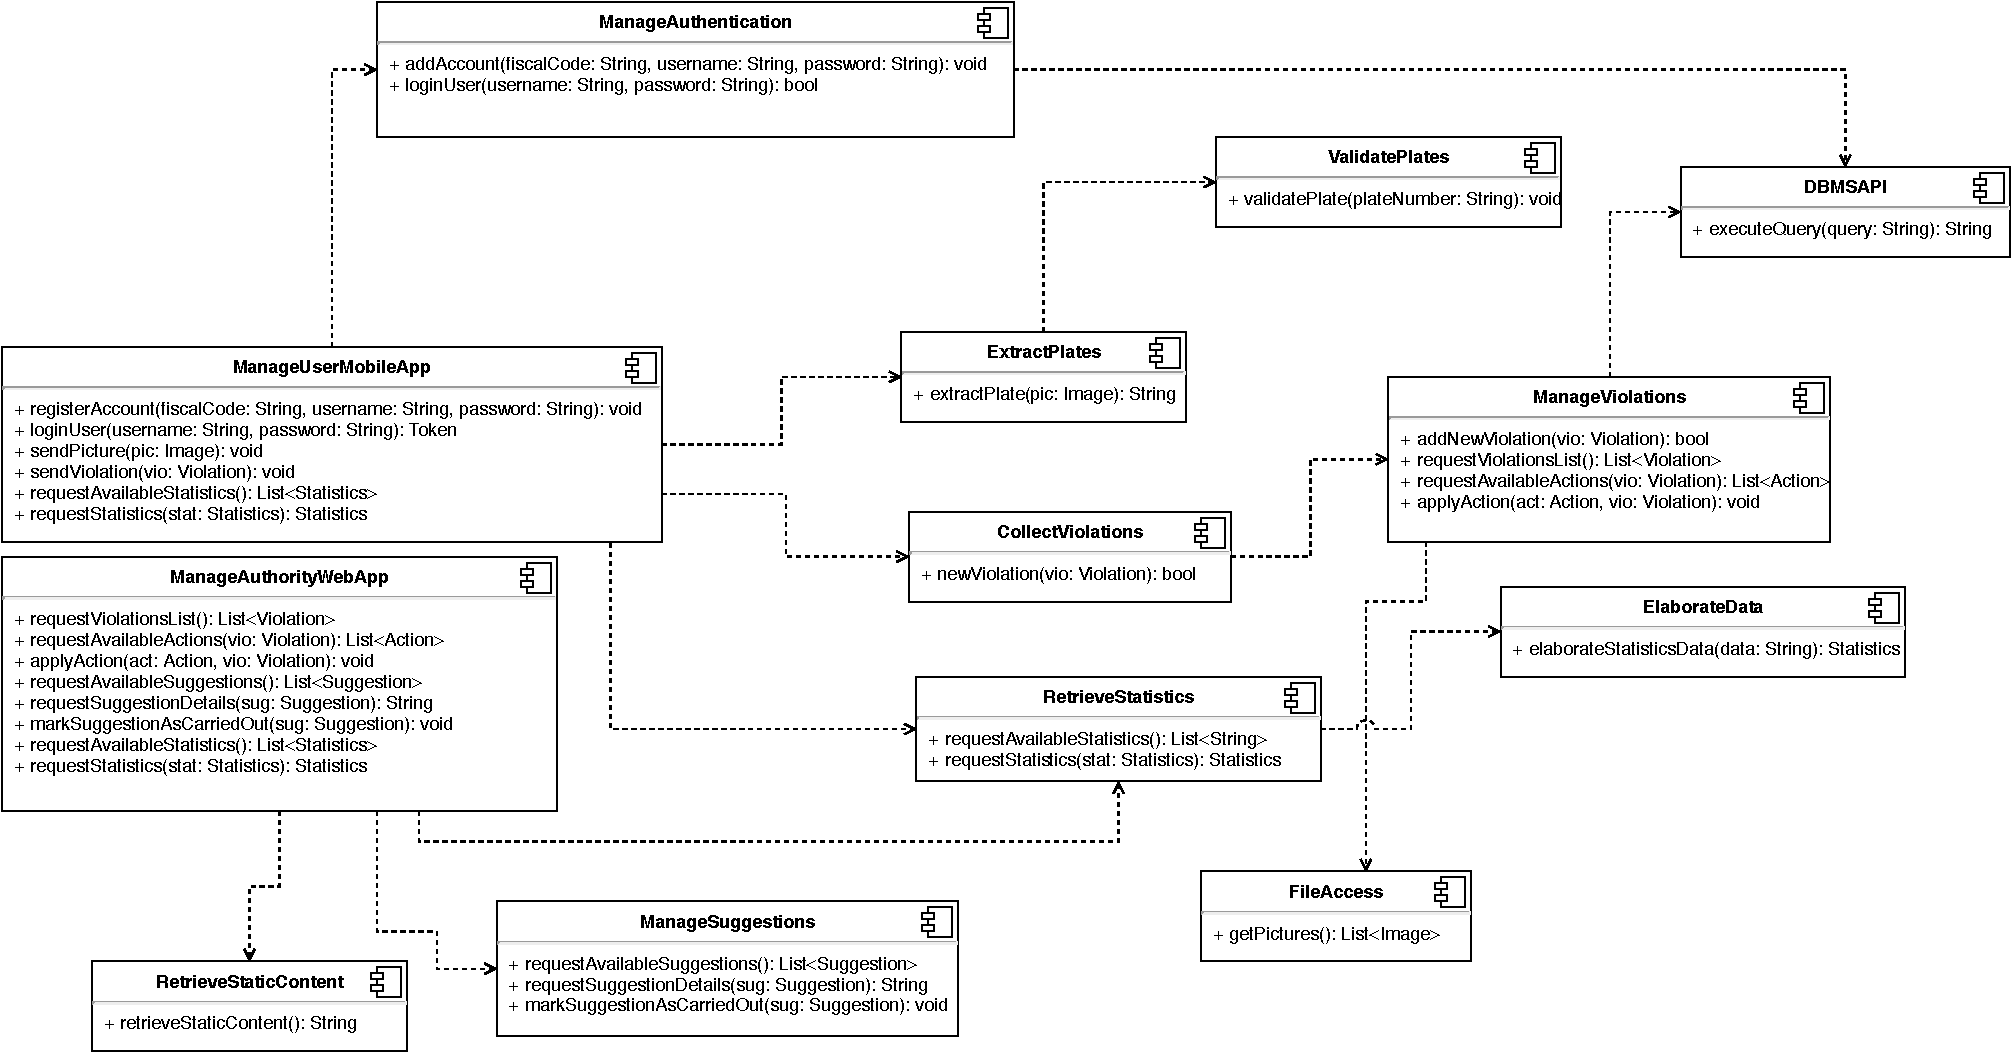
\includegraphics[width=\textwidth]{interface_diagram.pdf}
    \caption{Interfaces that are used in the Application Server}
    \label{fig:interface_diagram}
\end{figure}

\begin{figure}[ht]
    \centering
    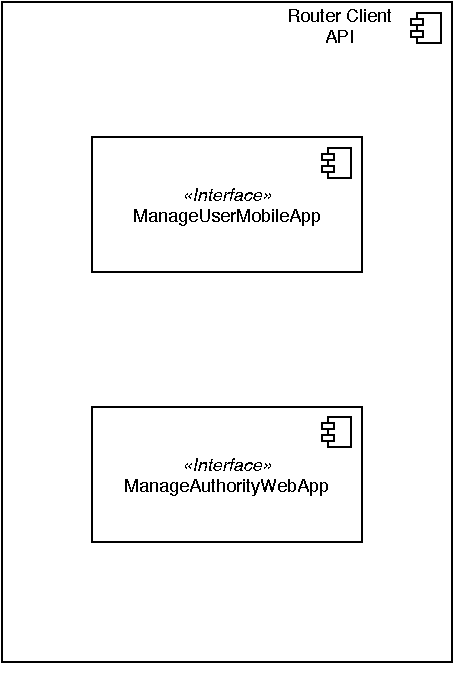
\includegraphics[width=5cm]{router_interface.pdf}
    \caption{Exploded view of the interface provided by the Router component}
    \label{fig:router_interface}
\end{figure}